% Drop-in LaTeX figure block for the Results section.
% Required preamble:
%   \usepackage{graphicx}
%   \usepackage{subcaption}
%   \graphicspath{{figures/}}
%
% Copy the corresponding PNG files from eval/results/figures/ and
% eval/runs/p3_sweep/sweep_energy_ratio.png into your paper's figures/ dir.

% =====================================================================
% Headline: productivity-survival tradeoff scatter
% =====================================================================
\begin{figure}[t]
  \centering
  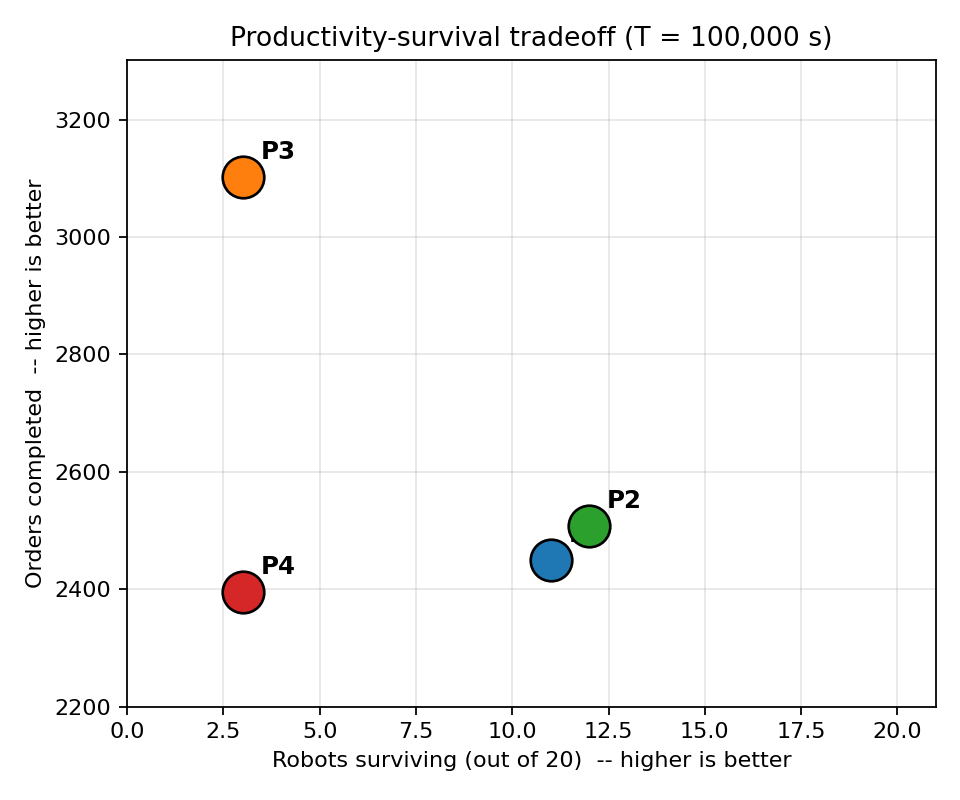
\includegraphics[width=0.85\columnwidth]{tradeoff.png}
  \caption{Productivity-survival tradeoff at the 100\,000\,s horizon.
  Each marker is one charger placement pipeline (12 chargers, 20 robots).
  P2 (Affinity Propagation) maximizes survivorship; P3
  (Picker-Tier) maximizes throughput; no pipeline dominates both axes.}
  \label{fig:tradeoff}
\end{figure}

% =====================================================================
% Two-panel: survivorship + throughput
% =====================================================================
\begin{figure*}[t]
  \centering
  \begin{subfigure}[t]{0.48\textwidth}
    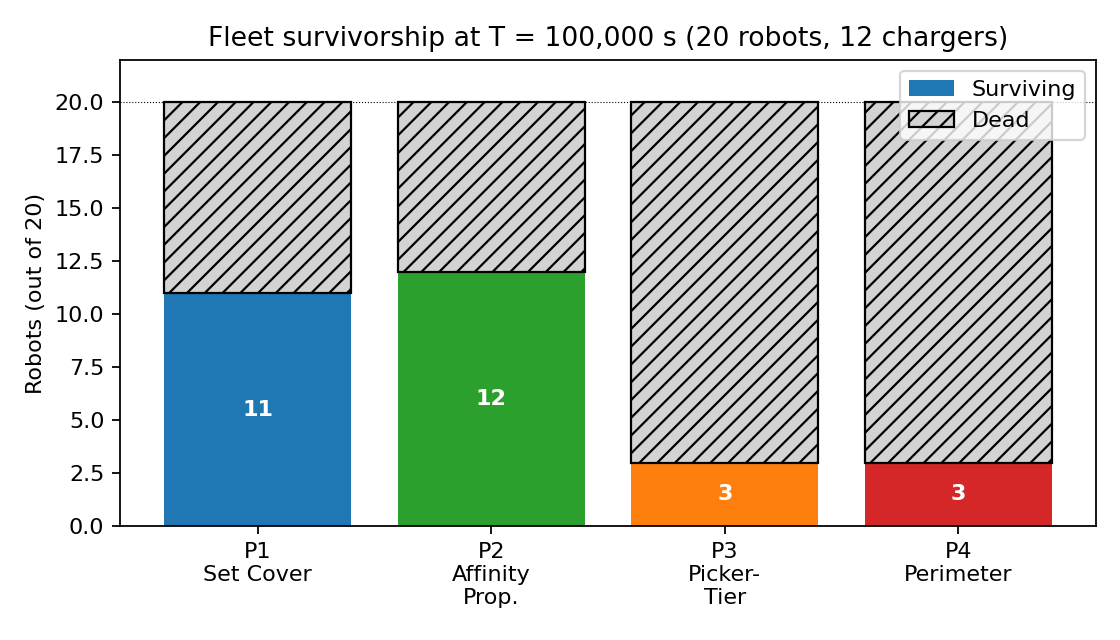
\includegraphics[width=\textwidth]{survivorship.png}
    \caption{Surviving robots after 100\,000\,s. Hatched portions
    represent fleet loss.}
    \label{fig:survivorship}
  \end{subfigure}
  \hfill
  \begin{subfigure}[t]{0.48\textwidth}
    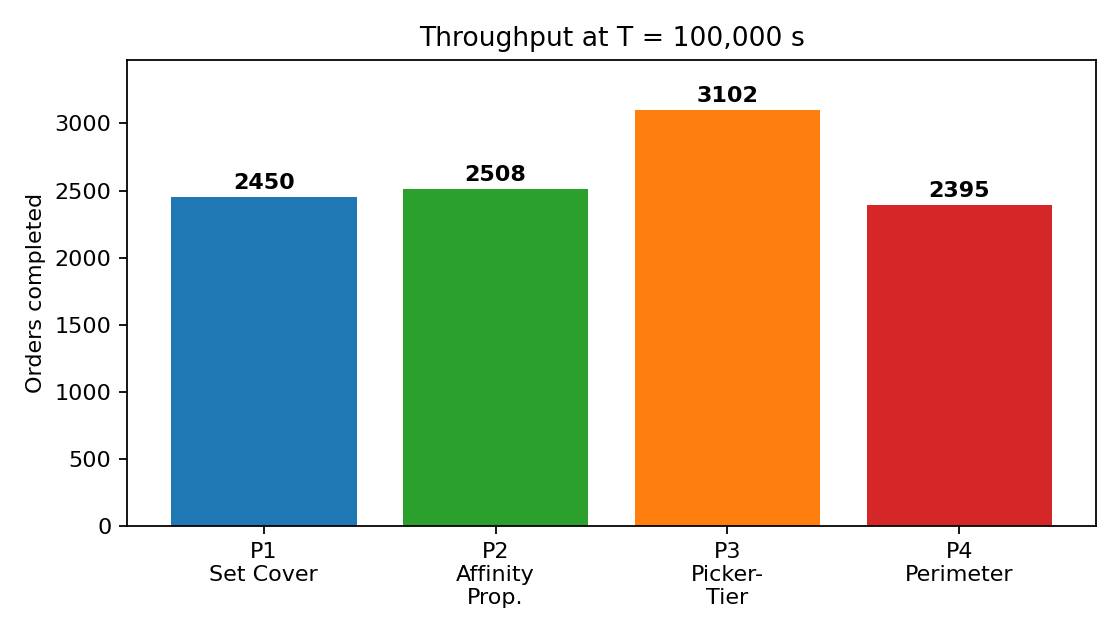
\includegraphics[width=\textwidth]{throughput.png}
    \caption{Orders completed across the same horizon. P3 is the
    productivity outlier despite lowest survivorship.}
    \label{fig:throughput}
  \end{subfigure}
  \caption{Two-axis breakdown of pipeline outcomes.
  Cluster-based placement (P2) preserves the fleet; dwell-aligned
  placement (P3) maximizes work but exhausts the fleet.}
  \label{fig:two_axis}
\end{figure*}

% =====================================================================
% Energy balance per pipeline
% =====================================================================
\begin{figure}[t]
  \centering
  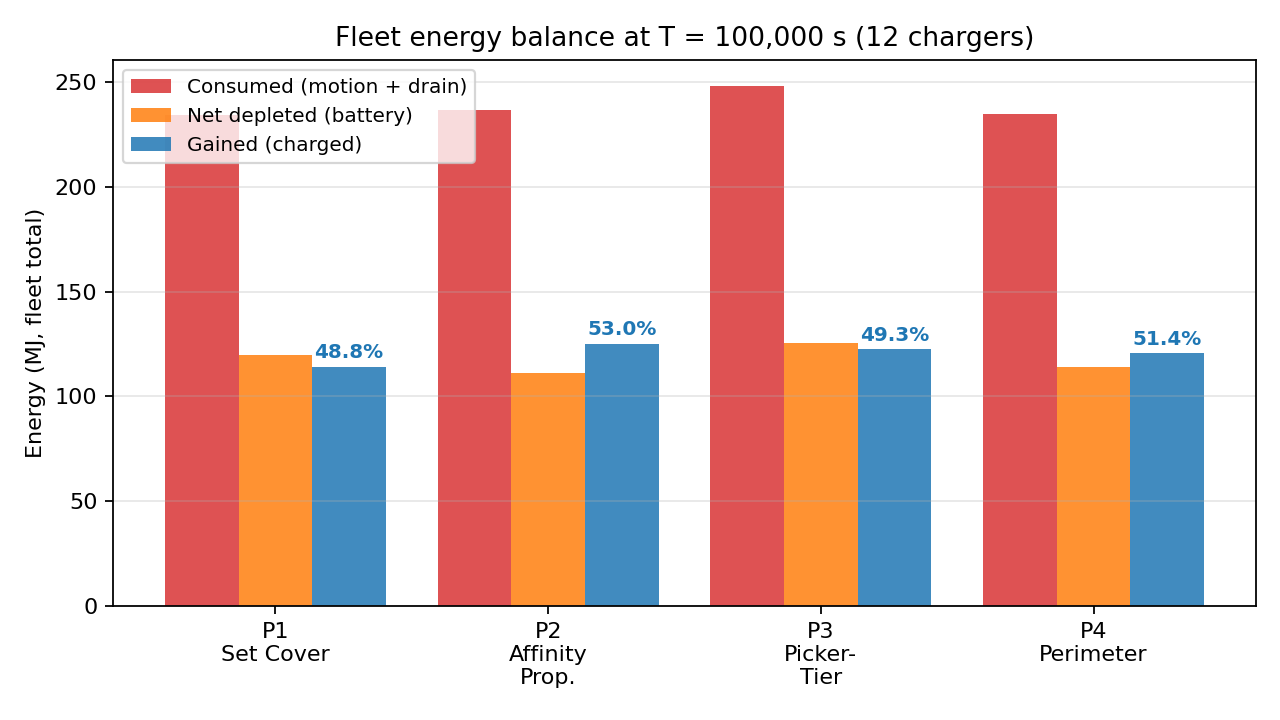
\includegraphics[width=0.95\columnwidth]{energy_balance.png}
  \caption{Fleet energy balance over the 100\,000\,s horizon.
  All four pipelines recover only 49--53\,\% of consumed energy,
  indicating that 12 chargers are insufficient regardless of placement.}
  \label{fig:energy_balance}
\end{figure}

% =====================================================================
% End-of-run state breakdown (optional, useful for discussion section)
% =====================================================================
\begin{figure}[t]
  \centering
  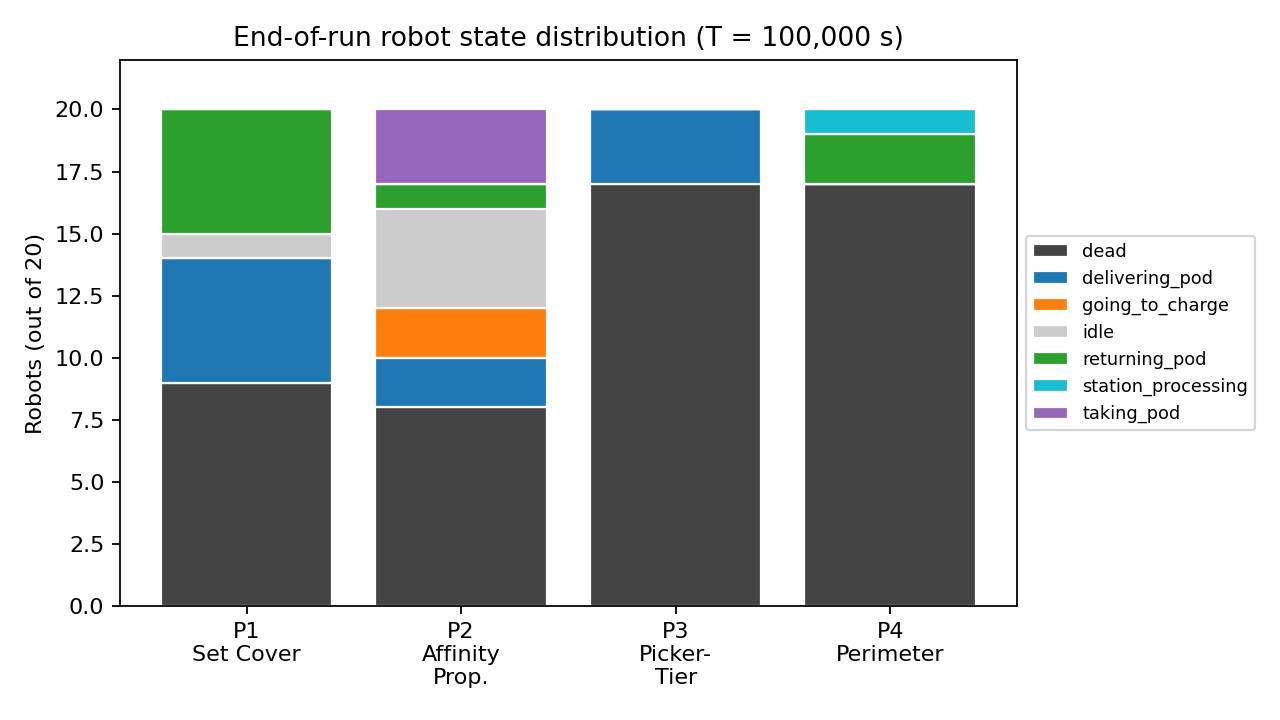
\includegraphics[width=0.95\columnwidth]{state_breakdown.png}
  \caption{End-of-run distribution of robot states. Dead robots
  (dark) dominate P3 and P4; only P2 retains a meaningful population
  in productive states (delivering / returning / taking pod).}
  \label{fig:states}
\end{figure}

% =====================================================================
% Charger-count sweep on P3 (20k horizon, separate experiment)
% =====================================================================
\begin{figure}[t]
  \centering
  
\includegraphics[width=\columnwidth]{sweep_energy_ratio.png}
  \caption{P3 charger-count sweep at 20\,000\,s. Replenish ratio
  improves with charger budget but never crosses 100\,\%, confirming
  diminishing returns up to 25 chargers.}
  \label{fig:sweep}
\end{figure}
